\documentclass[11pt,fleqn, oneside,openany]{book} % Default font size and left-justified equations

% use this list: https://www.educative.io/blog/google-coding-interview

%%%%%%%%%%%%%%%%%%%%%%%%%%%%%%%%%%%%%%%%%%%%
%               Structure
%%%%%%%%%%%%%%%%%%%%%%%%%%%%%%%%%%%%%%%%%%%%
\input{sources/preamble.tex}



\interfootnotelinepenalty=10000



\begin{document}

%\frontmatter
%\begingroup
%\thispagestyle{empty}
%\begin{tikzpicture}[remember picture,overlay]
%  \coordinate [below=12cm] (midpoint) at (current page.north);
%  \node at (current page.north west)
%  {\begin{tikzpicture}[remember picture,overlay]
%      \node[anchor=north west,inner sep=0pt] at (0,0) {\includegraphics[width=\paperwidth]{images/background}}; % Background image
%\textsl{}
%      \draw[anchor=north] (midpoint) node [fill=ocre!30!white,fill opacity=0.6,text opacity=1,inner sep=1cm]{\Huge\centering\bfseries\sffamily\parbox[c][][t]{\paperwidth}{\centering Coding Interview Essentials\\[15pt] % Book title
%      {\Large - }\\[20pt] % Subtitle
%      {\huge Davide Spataro}}}; % Author name
%    \end{tikzpicture}};
%\end{tikzpicture}
%\vfill
%\endgroup


\includepdf[pages={2},fitpaper=true]{images/book_covers1.pdf}



\usechapterimagefalse % If you don't want to include a chapter image, use this to toggle images off - it can be enabled later with \usechapterimagetrue

%\chapterimage{images/header} % Table of contents heading image
\pagestyle{empty} % No headers


\begin{center}
    \vspace*{2cm}
    
    {
        \Huge
        \test Coding Interview Essentials
    }
        
    \vspace{0.5cm}
     {
         %subtitle
     }
         
    \vspace{1.5cm}
    
    {
        \Large
        Davide Spataro
    }

    \vfill
             
  %  A thesis presented for the degree of\\
  %  Doctor of Philosophy
         
    \vspace{0.8cm}
  
    %\includegraphics[width=0.4\textwidth]{university}
         
 %   Department Name\\
 %   University Name\\
 %   Country\\
 %   Date
\end{center} 
    

\tikz[remember picture,overlay] \node[opacity=0.1,inner sep=0pt] at (current page.center){\includegraphics[width=\paperwidth,height=\paperheight]{images/cube.pdf}};

%\newpage

%\null\vfill
\noindent
Copyright \copyright \the\year\ Davide Spataro\par
Permission is granted to copy, distribute and/or modify this document under the terms of the LGPL, Version 3.0 or any later version published by the Free Software Foundation; with no Invariant Sections, no Front-Cover Texts, and no Back-Cover Texts. A copy of the license is included in the section "\nameref{license:gnu}" at page \pageref{license:gnu}. 
\clearpage





%\clearpage
\thispagestyle{plain}
\par\vspace*{.35\textheight}{\centering Dedicated to my \par}

\frontmatter

\tableofcontents % Print the table of contents itself

\chapter*{Preface}
\addcontentsline{toc}{chapter}{Preface}

Landing a lucrative job as a software engineer at FAANG is an increasingly competitive endeavour. It is not uncommon to have to go through and impress in 5 or more technical rounds, each of which will require you to solve complex coding problems in a high pressure environment. 

A common preparation strategy is to binge code on one of the many online coding platforms that cater to this need. This however, is not the optimal approach as the quality of the resources on these websites is insufficiently high or consistent to ensure the solid grasp of solution fundamentals needed to quickly adapt to the specifics of any question that may come up in real life.

For this reason, I have decided to take a different approach and, having spent several years studying the most common interview problems based on surveys from candidates, I have complied a subset of problems whose solutions can be applied across a broad array of actual interview questions. These problems and their solutions are presented in bite-sized quality lessons which will hopefully provide you with the tools you need to go on and succeed at interview. 


\medskip
\begin {flushright}
  Davide Spataro \hfill \\
  Amsterdam, The Netherlands, \today
\end {flushright}
\chapter*{Acknowlegements}
\addcontentsline{toc}{chapter}{Aknowledgments}


\chapter*{About the author}
\addcontentsline{toc}{chapter}{About the author}

\begin{wrapfigure}{r}{0.5\textwidth}
    \vspace{-20pt}
    \begin{center}
        \includegraphics[width=0.48\textwidth]{images/me_linkedin}
    \end{center}
    %\vspace{-20pt}
    %\caption{A gull}
    \vspace{-15pt}
  \end{wrapfigure}

He was born the 14th February 1990 and grew up in Nicotera, a small city in Southern Italy. He attended the secondary school focusing on humanities and in 2008 he moved to Cosenza, the city where  he studied and worked for 3 years collaborating with researchers of the Department of Mathematics and Computer Science on the modellation and simulation of complex natural systems. His research interests revolve around the central topic of "Parallel Computing" in the context of High-Performance Computing (HPC). Since 2018 he lives in Eindhoven where he works as Software Engineer at ASML working on TWINSCAN photolitography systems. He studied piano and music since he was eight for ten years, long enough to make him addicted to classical and jazz music. In 2011, he obtained the Bachelor of Science in Computer Science at the University of Calabria. and since 2014 he holds the Master of Science (summa cum laude) from the University of Calabria. Since April 2015 member of the NVIDIA GPU Educational Center at UNICAL.  In  January 2018 he succesfully defended his Ph.D. thesis with title: "Acceleration of numerical regular grid methods on manycore systems".  More information on his CV.


%I am a curious and passionate software engineer and my interests include, but are not %limited to, C++, parallel programming and GPGPU. I am an active StackOverflow user, %avid reader of technical and scientific books and articles. Participating in %competitive programming competitions, writing blog articles on C++ and algorithms and %doing online
%lesson, is how I keep challenging myself daily. I feel naturally inclined to work in a %team, but I am also capable of tackling and solving complex
%problems autonomously. In addition,
%I am always looking for people and
%experiences from which I can learn
%and improve. I was born and raised in
%Nicotera, Southern Italy. At the age of
%12 I started programming and I have
%studied piano and music for 10 years,
%long enough to make me addicted
%to classical and jazz music, until the
%age of 18 when I decided to concentrate fully on Computer Science.
%Besides that, I am passionate about
%photography and investing. When I
%am not coding I am most likely either
%paddling in the Mediterranean sea,
%lifting weights in the gym or fighting
%gravity on a race bike. I drink a lot of
%coffee 

\chapter*{A note from the author}
\addcontentsline{toc}{chapter}{A note from the author}

\section*{How I began writing this book}
I started writing what eventually become this manuscipt in 2018. 
Until then, I followed a quite strict daily study routine that consisted of solving at least one coding interview/competitive programming challenge and, only for those worth the effort, to put together a markdown document with a summary of the problem and all the solution approaches plus the thought process that lead me to them.

Therefore, right from the beginning, solving a coding interview question meant for me more than just writing solutions and unit-tests.
My main goal was writing code and notes, like short essays, that I could use to boostrap my understanding of the problem months or years later.
The idea I had in mind was that, when it was time to throw myself into a real interview I could use this material as a reference and sharpen my preparation with material 
that I was sure to be correct and I could absorb and understand quickly.

Over the years I accumulated a substantial amount of material that I eventually started sharing with colleagues at the university and at work. 
Many of them found the content and the format of my notes useful and convinced me to polish, add illustrations and organize them into a proper collection.

\section*{C++ as language of choice}
Almost all the solution code in this book is written in C++ (C++14/17/20 and newer version). 
I have been using C++ academically and professionally since I basically started programming and the original material I have collected over the years was almost entirely C++ code. 
The reason I did not decide to rewrite it in another language is that C++ is still nowadays an extremely popular language and engineers skilled in this language are in big demand which, in turn means that C++ is very much used in interviews!
Moreover, C++ is also one of the most adopted languages in the competitive programming community and this makes it easier to find resources on problems.

I tried my best to stick to standard C++ and not to use any compiler specific features so that it is easy to port every piece of code in this book to different mainstream imperative language like C\#, Python or Java.  
Eventually during an interview you need to code (hopefully elegant, fast and readable) solutions, but, without the right algorithm, these would be vain efforts. Therefore the focus of this book is more on trying to convey the insights and core ideas of the best algorithms and not on a particular feature of a particular programming languages.
This does not mean the code you will find in this book is sloppy or C++ unidiomatic. Quite the opposite, I tried to make full use of the its potential.

All the solutions have been compiled and tested using \inline{gcc (GCC) 11.1.0} and \inline{clang version 12.0.1} but I am confident they will compile and work on other toolchain/system. 

\section*{Organization}
I always try to be consistent in the way I approach a problem:
\begin{enumerate}
    \item I start by looking at a few examples and to think about corner cases and unclarities in the problem statement that I could address by asking questions to the interview.
    \item When I was comfortable with my understanding of the problem, I start thinking in general about the problem by for instance trying to find similarities with other problems I solved in the past or figuring out a lower bound.
    \item I would then move into summarizing (usually only on paper) the simplest (which is usually the slowest) solution I could think of; this would usually be some sort of brute-force that I can somehow derive from the statement itself.
    \item  From there I would try to think whether the brute-force solution can improved and be fast enough to be considered good or if I needed to shift my thinking towards other directions.
\end{enumerate}
Clearly these steps are not set in stone and sometime I knew right away what the optimal solution is. 
For the majority of the cases tough, I would go through most of the steps above and this is the reason why each chapter has pretty much the same sections organization where we have:
\begin{itemize}
    \item \textit{\quotes{Introduction}}, where I set the stage for the problem.
    \item A section \textit{\quotes{Problem statement}} enunciating the formal statement for the problem;
    \item \textit{\quotes{Discussion}}, where I make the firsts observations and deductions that I can use later when crafting solutions.
    The rest of this Section is usually followed by a number of subsection each describing in detail a solution. These subsections are (as much as possible) sorted by descreasing time complexity, space used and simplicity/readibility and ease of implementation. 
 \end{itemize}

I believe that coding interviews have a lot of similarities with sport competitions. If you train to be a good tennis player you reharse the same movement over and over again. Interviews are no different. 
Interviewers are not expecting candidates to be silent and just write code like machines; 
You need to show your thought process along the entire interview and being comfortable in doing so in a high pressure situation. This is where having a method that you reharsed over and over helps. I  belive the chapter's arrangements of the sections is functional to this goal and that you can use it to reharse solving a problem like you are guiding the interviewer along with you on a journey from the slowest to the best solution. 


\section*{Rest}
Write as if you spoke directly to your readers about your written work.
preparing 
Short summary of the book. 
How did you decide to write this book? You started off with a set of notes and written code. you noticed that were useful to others and slowly decided to organize them and add illustrations to it. this is how it started. 

Why did you decide to go for c++ and not another language? Consider that the ideas and code in the text can be easily ported to other mainstream languages. I tried my best not to introduce any language/compiler/system specific instructions of hacks.

It is important to remember this is a book about coding interview and not on algorithm. 
identify significant omissions, abridgments, simplifications, or inventions; 


what was the writing process?
creation process, including composition, revision, research, challenges, and impactful events along the way. personal growth and learning through the writing process; 
Recount challenges while writing => create illustrations that were able to integrate the text and the code was not easy. 


The author’s note can be used to give credit where credit is due by acknowledging individuals’ contributions, references, and other’s materials included in the core text.

How is the book organised? Why this specific organization?


\section*{Audience}






\mainmatter




%\lstlistoflistings
%\listoffigures
%\listoftables

%\cleardoublepage % Forces the first chapter to start on an odd page so it's on the right

%pagestyle{fancy} % Print headers again



%%%%%%%%%%%%%%%%%%%%%%%%%%%%%%%%%%%%%%%%%%%%
%               Appendices
%%%%%%%%%%%%%%%%%%%%%%%%%%%%%%%%%%%%%%%%%%%%

\chapter*{Appendices}
\addcontentsline{toc}{chapter}{Appendices}
% @Author: Davide Spataro
% @Date:   2020-10-25 
% @Last Modified by:   Davide Spataro

\section{Dynamic Programming}
\label{sect:appendix:DP}

Dynamic programming (DP) is a popular tecnique for solving a certain class of
optimization problems efficiently and is accredited to the American Scientist
Richard Bellman\cite{bellman1954}. The word \textit{programming} can be a bit deceiving for
computer scientist of programmers in general but it has really little to do with
computer programming and it is infact intended as a set of rules to 
follow to solve a certain problem. These rules can of course be coded and
executed by a computer but can be easily followed on paper for instance. 
Dynamic programming is better thought as an optimization approach rather than an
method or framework where a complex optimization problem is transformed into a sequence of
smaller (and simpler) problems. The very essence of DP is its multi-stage
optimization procedure. DP does not provide directly with the
instruction on how to solve a particular problem, but instead provides a general
framework that requires creativity and non trivial effort/insights so that a
problem formulation can be adapted and casted within the DP framework bounds.
This is possibly the reason why DP is considered a rather hard topic and it is
particularly feared during interviews. 

This chapter is not intended to be a full treatement of DP, and we will
introduce and describe it to the level that is necessary to understand and
better tackle DP interview problems. For a more comprenshive material on DP
please refer to \cite{bellman1954, cormen2009}.


\section*{Listings}

\lstinputlisting[language=c++, caption={ Functor used to calculate the hash value for a pair of integers.     \inline{hash_combine} is a free function used to mix several input hash values into a new one.  },label=list:listings:hash_pair]{/home/dspataro/git/algorithm_articles/test/common/hash_pair.h}
%\section{Prefix sum}
In computer science, the prefix sum, cumulative sum, inclusive scan, or simply scan of a sequence of numbers x0, x1, x2, ... is a second sequence of numbers y0, y1, y2, ..., the sums of prefixes (running totals) of the input sequence:
%% @Author: Davide Spataro
% @Date:   2020-03-30 17:18:14
% @Last Modified by:   Davide Spataro
% @Last Modified time: 2020-03-30 17:28:08
\section{Binary Search}
\label{sect:appendix:binary_search}
\lipsum{1}
%%%%%%%%%%%%%%%%%%%%%%%%%%%%%%%%%%%%%%%%%%%%
%               BIBLIOGRAPHY
%%%%%%%%%%%%%%%%%%%%%%%%%%%%%%%%%%%%%%%%%%%%

%
%from documentation
%\newacronym[⟨key-val list⟩]{⟨label ⟩}{⟨abbrv ⟩}{⟨long⟩}
%above is short version of this
% \newglossaryentry{⟨label ⟩}{type=\acronymtype,
% name={⟨abbrv ⟩},
% description={⟨long⟩},
% text={⟨abbrv ⟩},
% first={⟨long⟩ (⟨abbrv ⟩)},
% plural={⟨abbrv ⟩\glspluralsuffix},
% firstplural={⟨long⟩\glspluralsuffix\space (⟨abbrv ⟩\glspluralsuffix)},
% ⟨key-val list⟩}

\newacronym{cd}{CD}{compact disk}
\newacronym{utc}{UTC}{Coordinated Universal Time}
%\newacronym{adt}{ADT}{Atlantic Daylight Time}
%\newacronym{est}{EST}{Eastern Standard Time}
 
% Use the acronyms
\gls{utc} is 3 hours behind \gls{adt} and 10 hours ahead of \gls{est}.



%\addcontentsline{toc}{chapter}{\textcolor{ocre}{Glossary}}
%\printglossaries


%Print the glossary

\addcontentsline{toc}{chapter}{\textcolor{ocre}{Bibliography}}
%\chapter*{Bibliography}
%Print the glossary
\printbibliography	


%%%%%%%%%%%%%%%%%%%%%%%%%%%%%%%%%%%%%%%%%%%%
%               LICENSE
%%%%%%%%%%%%%%%%%%%%%%%%%%%%%%%%%%%%%%%%%%%%	
\input{sources/license.tex}
\addcontentsline{toc}{chapter}{GNU LESSER GENERAL PUBLIC LICENSE}


%%%%%%%%%%%%%%%%%%%%%%%%%%%%%%%%%%%%%%%%%%%%
%               INDEX
%%%%%%%%%%%%%%%%%%%%%%%%%%%%%%%%%%%%%%%%%%%%	
	\cleardoublepage
	\phantomsection
	\setlength{\columnsep}{0.75cm}
	\addcontentsline{toc}{chapter}{\textcolor{ocre}{Index}}
	\printindex


	%\backmatter


\end{document}
